\documentclass[twocolumn]{article}
\usepackage[margin=.8in]{geometry}
\usepackage{listings}
\usepackage{longtable}
\usepackage{booktabs}
\usepackage{graphicx}
\usepackage{subcaption}
\usepackage{hyperref}

\newcommand{\colAwidth}{0.2\textwidth}
\newcommand{\colBwidth}{0.73\textwidth}

\newcounter{datadefnum} %Datadefinition Number
\newcommand{\ddthedatadefnum}{DD\thedatadefnum}
\newcommand{\ddref}[1]{DD\ref{#1}}


\title{Research Topic Handout -- Examples}
\author{Daniel Szymczak\\
McMaster University}
\date{June 28, 2018}

\begin{document}

\maketitle
{\noindent\emph{Note: This handout was created as a companion-piece to my 
supervisory committee meeting presentation for June 28, 2018}}

\section{Too much duplication!}

In any piece of software, the same knowledge will appear across many different 
artifacts. Manually entering this knowledge multiple times
increases the potential for errors to occur.

From our case study on a fuel pin in a nuclear reactor, we see $h_g$~--~a 
symbol which appears in the Software Requirements Specification (SRS), the 
Literate Programmer's Manual (LPM), and the source code.

The following table shows a (simplified) definition of $h_g$ taken from the 
SRS.

\noindent
\begin{minipage}{0.4\textwidth}
\begin{tabular}{p{\colAwidth} p{\colBwidth}}
\toprule
\textbf{Number} & \textbf{DD\refstepcounter{datadefnum}\thedatadefnum} 
\label{hg}\\
\midrule
Label & $h_g$\\
\midrule
Equation & $h_g$ =$ \frac{2k_{c}h_{p}}{2k_{c}+\tau_c h_{p}}$\\
\midrule
Description & $h_g$ is the  gap conductance \dots \\
\midrule
\dots & \\
\bottomrule
\end{tabular}
\end{minipage}\\

\begin{equation}
\label{E:h.g} 
h_{g} =\frac{2k_{c}h_{p}}{2k_{c}+\tau_c h_{p}}
\end{equation}

The defining equation for $h_g$ also appears in Equation~\ref{E:h.g}, taken 
from the LPM, and it appears again in the corresponding C code:

\begin{lstlisting}[basicstyle=\scriptsize]
double calc_hg(double k_c,double h_b,double tau_c)
{
 return (2*k_c*h_p) / ((2*k_c) + (tau_c * h_p));
}
\end{lstlisting}

This kind of duplication is all too common and writing one piece of information 
in multiple places is tedious and time-consuming. Wouldn't it make more sense 
to encode a definition once and automatically reuse it wherever required in 
our software artifacts?

\section{Inter-/intra-artifact\\consistency}
\label{Sec:consistency}

Our five case studies have been reviewed at least once per year by multiple 
people. Every time the documents are reviewed, new inconsistencies and problems 
with the artifacts are found. We show a subset of the 
issues that are currently open (Figure~\ref{Fig:OpenIssues}), 
\begin{figure}
  \centering
  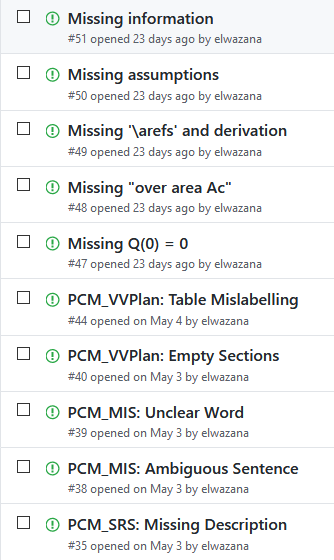
\includegraphics[width=0.7\linewidth]{OpenIssuesSWHS.PNG}
  \caption{Subset of the currently open issues with PCM}
  \label{Fig:OpenIssues}
\end{figure}
or closed within 
the last two months (Figure~\ref{Fig:ClosedIssues}) for \emph{one} 
particular case study -- the Solar Water Heating System with Phase Change 
Material, also known as PCM -- but similar issues have been found across all of 
our case studies. If you would like to see more, the PCM case study is publicly 
accessible at \url{https://github.com/smiths/swhs}.
\begin{figure}[!htbp]
  \centering
  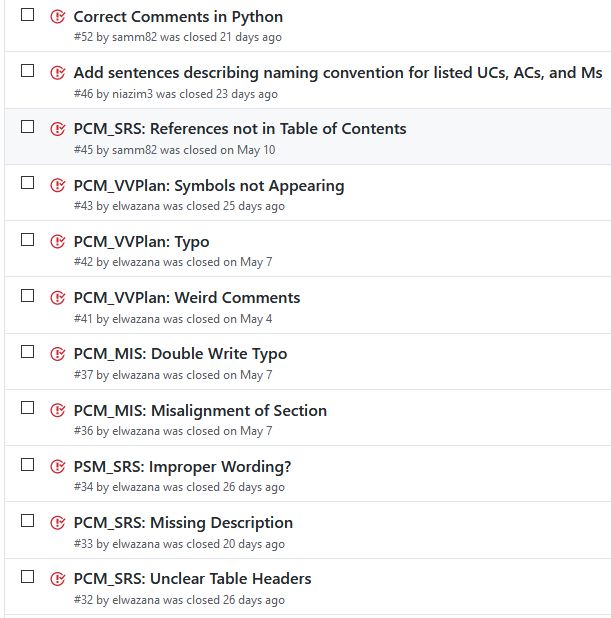
\includegraphics[width=\linewidth]{RecentIssuesSWHS.PNG}
  \caption{Closed issues within the last two months}
  \label{Fig:ClosedIssues}
\end{figure}

Each of those issues is related to some inconsistency found in the 
manually-produced software artifacts. Information is missing, out of date, 
unclear, or simply incorrect. Every closed issue from 
Figure~\ref{Fig:ClosedIssues} had to be taken care of manually and took a 
non-trivial amount of time.

It is easy to see a problem exists with maintaining consistent artifacts. 
Changes made to the code, requirements, or design do not always have obvious 
repercussions (inter-artifacts) and inconsistencies can begin to appear. Code 
and documentation reviews allow us to find some such inconsistencies, but the 
majority of them should be avoidable in the first place if there were some way 
to test the effects of a change. Why do we build automated tests for code, but 
not other software artifacts? Why not automatically trace our 
artifacts and report where a given change will affect them? What if we could 
ensure consistency by construction?

\emph{Note: An example of intra-artifact consistency will be covered on slides 
\#25-30 in the companion presentation.}

\section{Design for change}

Consider the PCM case study mentioned in Section~\ref{Sec:consistency}. It is a 
single member of a larger software family. If we decide to remove the phase 
change material from the problem, our solution will still be very similar with 
the obvious lack of any information related to phase change material -- it 
becomes the noPCM case study.

A lot of PCM's design can (and should) be reused for noPCM. Not only that, but 
if we have designed the system with change in mind, it should be easy, if not 
trivial, to switch from PCM to noPCM. Why not make it easier to target software 
families instead of singular family members?

\section{(Re-)Certification is expensive}

Software certification is necessary by law in certain fields, particularly in 
safety-critical applications. Certifying bodies exist across domains 
and each have their own list of requirements. Looking at some 
examples \cite{CDRH2002,CSA1999,CSA2009,FDA2014} there are many common  
requisite documentation artifacts including, but not limited to:

\begin{itemize}
\itemsep-.2em
\item Problem definition
\item Theory manual
\item Requirements specification
\item Design description
\item Verification and Validation (V\&V) report
\end{itemize}

Overall certification is an expensive process. The exact costs can be hard to 
estimate~\cite{HatcliffEtAl2009}, but many person-hours are spent 
working on ensuring full traceability and consistency between software 
artifacts. Getting re-certified should anything need to be updated is a 
similarly long and costly process as all artifacts must be updated and 
re-verified manually.

While we are not proposing to automatically verify our software artifacts, we 
want to relieve the burden of artifact creation. What if instead of manually 
maintaining each artifact, we could automatically generate them? 

\bibliographystyle{abbrv}
\bibliography{drasil}  
\end{document}
